\textbf{TensorFlow} es una plataforma de código abierto para crear y usar modelos de aprendizaje automático. Implementa muchos de los algoritmos y patrones comunes necesarios para el aprendizaje automático, lo que le evita tener que aprender todas las matemáticas y la lógica subyacentes y le permite concentrarse solo en su escenario. Está dirigido a todos, desde aficionados hasta desarrolladores profesionales e investigadores que superan los límites de la inteligencia artificial. Es importante destacar que también admite la implementación de modelos en la web, la nube, dispositivos móviles y sistemas embebidos.

\begin{figure}[htb]
	\centering
	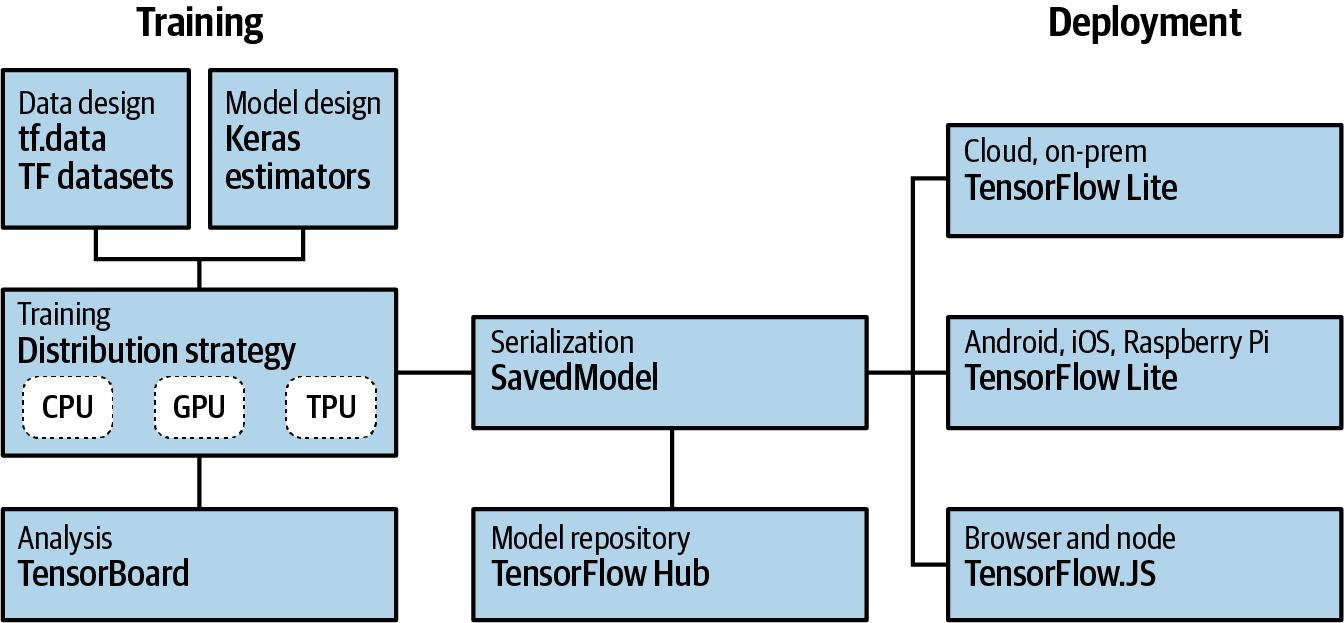
\includegraphics[width=0.7\textwidth]{capitulo3/TFarquitectura.jpg}
	\caption{Estructura de alto nivel de \textbf{Tensorflow}}
	\label{cap3:001}
\end{figure} 

El proceso de creación de modelos de aprendizaje automático se llama \textbf{entrenamiento}. Aquí es donde una computadora usa un conjunto de algoritmos para aprender sobre las entradas y lo que las distingue entre sí. Entonces, por ejemplo, si desea que una computadora reconozca gatos y perros, puede usar muchas imágenes de ambos para crear un modelo, y la computadora usará ese modelo para tratar de descubrir qué hace que un gato sea un gato y qué hace que un perro sea un perro. Una vez que se entrena el modelo, el proceso de reconocimiento o categorización de entradas futuras se denomina \textbf{inferencia}.

Entonces, para los modelos de entrenamiento, hay varias cosas que necesita admitir. Primero hay un conjunto de API para diseñar los propios modelos. Con TensorFlow, hay tres formas principales de hacer esto: 
\begin{itemize}
	\item Puede codificar todo a mano, donde descubre la lógica de cómo una computadora puede aprender y luego implementarla en el código (no recomendado)
	\item Puede usar estimadores integrados, que son redes neuronales ya implementadas que puede personalizar
	\item O puede usar Keras, una API de alto nivel que le permite encapsular paradigmas comunes de aprendizaje automático en el código
\end{itemize}

Hay muchas maneras de entrenar a un modelo. En su mayor parte, probablemente solo use un solo chip, ya sea una unidad de procesamiento central (CPU), una unidad de procesamiento de gráficos (GPU) o algo nuevo llamado unidad de procesamiento de tensor (TPU). En entornos de trabajo e investigación más avanzados, se puede utilizar la capacitación paralela en múltiples chips, empleando una estrategia de distribución en la que la capacitación abarca múltiples chips. TensorFlow también es compatible con esto.

Hay muchas maneras de entrenar a un modelo. En su mayor parte, probablemente solo use un solo chip, ya sea una unidad de procesamiento central (CPU), una unidad de procesamiento de gráficos (GPU) o algo nuevo llamado unidad de procesamiento de tensor (TPU). En entornos de trabajo e investigación más avanzados, se puede utilizar la capacitación paralela en múltiples chips, empleando una estrategia de distribución en la que la capacitación abarca múltiples chips. TensorFlow también es compatible con esto.

El elemento vital de cualquier modelo son sus datos. Como se discutió anteriormente, si desea crear un modelo que pueda reconocer gatos y perros, debe entrenarse con muchos ejemplos de gatos y perros. Pero, ¿cómo puedes manejar estos ejemplos? Verá, con el tiempo, que esto a menudo puede implicar mucha más codificación que la creación de los propios modelos. TensorFlow se envía con API para tratar de facilitar este proceso, llamado TensorFlow Data Services. Para el aprendizaje, incluyen muchos conjuntos de datos preprocesados que puede usar con una sola línea de código. También le brindan las herramientas para procesar datos sin procesar para que sea más fácil de usar.

Más allá de crear modelos, también deberá poder ponerlos en manos de las personas donde puedan usarse. Con este fin, TensorFlow incluye API para servir, donde puede proporcionar inferencia de modelos a través de una conexión HTTP para usuarios web o de la nube. Para que los modelos se ejecuten en sistemas móviles o integrados, existe TensorFlow Lite, que proporciona herramientas para la inferencia de modelos en Android e iOS, así como sistemas integrados basados en Linux, como Raspberry Pi. Una bifurcación de TensorFlow Lite, llamada TensorFlow Lite Micro (TFLM), también proporciona inferencia sobre microcontroladores a través de un concepto emergente conocido como TinyML. Finalmente, si desea proporcionar modelos a su navegador o a los usuarios de Node.js, TensorFlow.js ofrece la capacidad de entrenar y ejecutar modelos de esta manera. A continuación, le mostraré cómo instalar TensorFlow para que pueda comenzar a crear y usar modelos ML con él.

\section{Usando Tensorflow}

Veremos las tres formas principales en las que puede instalar y usar TensorFlow. Comenzaremos con cómo instalarlo en su caja de desarrollador usando la línea de comando. Luego exploraremos el uso del popular PyCharm IDE (entorno de desarrollo integrado) para instalar TensorFlow. Finalmente, veremos Google Colab y cómo se puede usar para acceder al código de TensorFlow con un backend basado en la nube en su navegador.


\subsection{Instalando Tensorflow en python}


TensorFlow admite la creación de modelos usando varios lenguajes, incluidos Python, Swift, Java y más. En este libro nos centraremos en el uso de Python, que es el lenguaje de facto para el aprendizaje automático debido a su amplia compatibilidad con modelos matemáticos. Si aún no lo tiene, le recomiendo encarecidamente que visite Python para empezar a utilizarlo y learnpython.org para aprender la sintaxis del lenguaje Python. Con Python, hay muchas formas de instalar marcos, pero la predeterminada que admite el equipo de TensorFlow es pip. Entonces, en su entorno de Python, instalar TensorFlow es tan fácil como usar:

\begin{lstlisting}[language=bash]
conda create -n tensorflow
conda activate tensorflow
pip install tensorflow
\end{lstlisting}

En el caso de que se quisiera borrar un ambiente de python debemos ejecutar:

\begin{lstlisting}[language=bash]
	conda deactivate
	conda env remove --name tensorflow
\end{lstlisting}

Una vez que esté en funcionamiento, puede probar su versión de TensorFlow con el siguiente código:

\begin{lstlisting}[language=bash]
import tensorflow as tf
print(tf.__version__)
\end{lstlisting}

\section{Usando tensorflow en PyCharm}

Me gusta especialmente usar la versión comunitaria gratuita de PyCharm para crear modelos con TensorFlow. PyCharm es útil por muchas razones, pero una de mis favoritas es que facilita la administración de entornos virtuales. Esto significa que puede tener entornos de Python con versiones de herramientas como TensorFlow que son específicas para su proyecto en particular. Entonces, por ejemplo, si desea usar TensorFlow 2.0 en un proyecto y TensorFlow 2.1 en otro, puede separarlos con virtual.

Me gusta especialmente usar la versión comunitaria gratuita de PyCharm para crear modelos con TensorFlow. PyCharm es útil por muchas razones, pero una de mis favoritas es que facilita la administración de entornos virtuales. Esto significa que puede tener entornos de Python con versiones de herramientas como TensorFlow que son específicas para su proyecto en particular. Entonces, por ejemplo, si desea usar TensorFlow 2.0 en un proyecto y TensorFlow 2.1 en otro, puede separarlos con entornos virtuales y no tener que lidiar con la instalación o desinstalación de dependencias cuando cambia. Además, con PyCharm puede realizar una depuración paso a paso de su código Python, algo imprescindible, especialmente si recién está comenzando. Por ejemplo, en la Figura 1-13 tengo un nuevo proyecto que se llama ejemplo1 y estoy especificando que voy a crear un nuevo entorno usando Conda. Cuando cree el proyecto, tendré un nuevo entorno virtual de Python limpio en el que puedo instalar cualquier versión de TensorFlow que desee (ver figura \ref{cap3:002}).

\begin{figure}[htb]
	\centering
	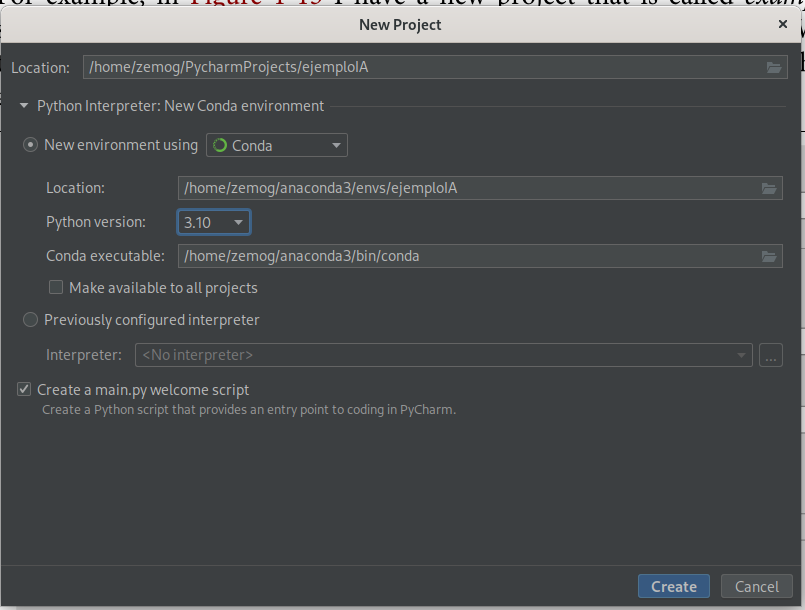
\includegraphics[width=0.7\textwidth]{capitulo3/creacion.png}
	\caption{Creación de un proyecto en PyCharm}
	\label{cap3:002}
\end{figure}

Una vez que haya creado un proyecto, puede abrir el cuadro de diálogo Archivo → Configuración y elegir la entrada ``Proyecto: <nombre de su proyecto>'' en el menú de la izquierda. Luego verá opciones para cambiar la configuración del Intérprete del proyecto y la Estructura del proyecto. Elija el enlace \textbf{Project Interpreter} y verá el intérprete que está utilizando, así como una lista de paquetes que están instalados en este entorno virtual, ver figura \ref{cap3:003}.



\begin{figure}[htb]
	\centering
	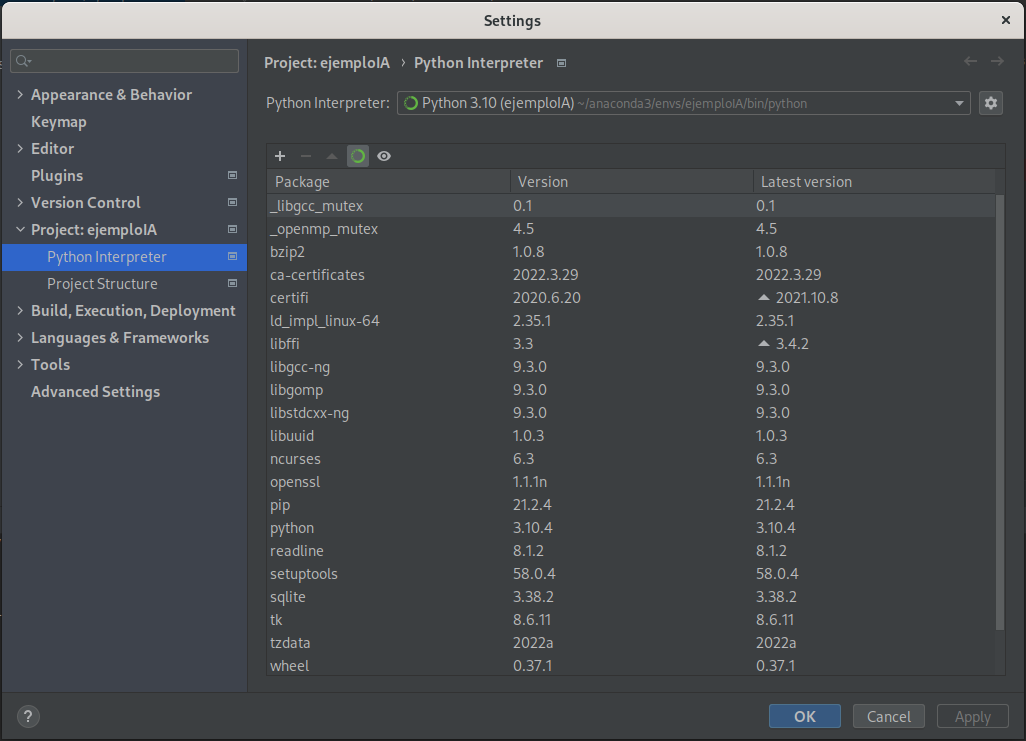
\includegraphics[width=0.7\textwidth]{capitulo3/agregarTensorflow.png}
	\caption{Agregando paquetes al ambiente virtual de python}
	\label{cap3:003}
\end{figure}


Haga clic en el botón + en la parte superior y se abrirá un cuadro de diálogo que muestra los paquetes que están disponibles actualmente. Escriba "tensorflow" en el cuadro de búsqueda y verá todos los paquetes disponibles con "tensorflow" en el nombre (figura \ref{cap3:004}). Una vez que haya seleccionado TensorFlow, o cualquier otro paquete que desee instalar, y luego haga clic en el botón Instalar paquete, PyCharm hará el resto.

instalaPaquete.png

\begin{figure}[htb]
	\centering
	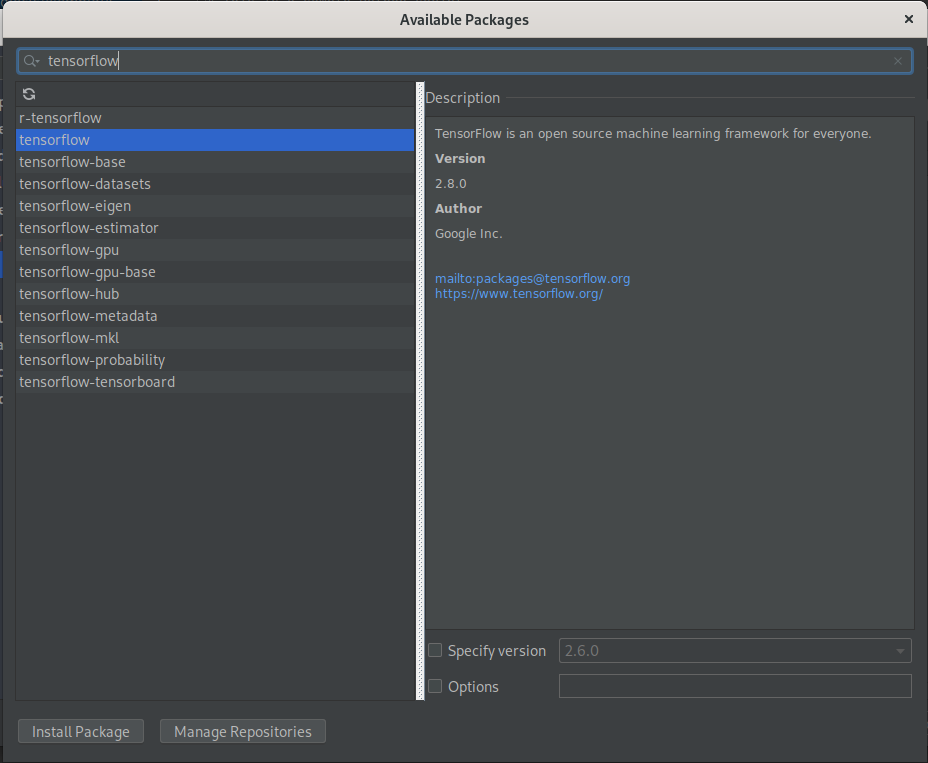
\includegraphics[width=0.7\textwidth]{capitulo3/instalaPaquete.png}
	\caption{Instalando Tensorflow en PyCharm}
	\label{cap3:004}
\end{figure}

Una vez que se instala TensorFlow, ahora puede escribir y depurar su código de TensorFlow en Python.

\section{Primeros pasos con el aprendizaje automático}

Como vimos anteriormente, el paradigma de aprendizaje automático es uno en el que tiene datos, esos datos están etiquetados y desea descubrir las reglas que hacen coincidir los datos con las etiquetas. El escenario más simple posible para mostrar esto en el código es el siguiente. Considere estos dos conjuntos de números:

\begin{lstlisting}[language=python]
xs = np.array([-1.0, 0.0, 1.0, 2.0, 3.0, 4.0], dtype=float)
ys = np.array([-3.0, -1.0, 1.0, 3.0, 5.0, 7.0], dtype=float)
\end{lstlisting}

aquí hay una relación entre los valores de \textbf{X} e \textbf{Y} (por ejemplo, si X es -1, entonces Y es -3, si X es 3, entonces Y es 5, y así sucesivamente). ¿Puedes verlo? Después de unos segundos, probablemente vio que el patrón aquí es \textbf{Y = 2X – 1}. ¿Cómo obtuvo eso? Diferentes personas lo resuelven de diferentes maneras, pero normalmente escucho la observación de que X aumenta en 1 en su secuencia e Y aumenta en 2; así, \textbf{Y = 2X +/– algo}. Luego observan cuando X = 0 y ven que Y = –1, por lo que calculan que la respuesta podría ser \textbf{Y = 2X – 1}. Luego observan los otros valores y ven que esta hipótesis “encaja”, y la respuesta es \textbf{Y = 2X – 1}. Eso es muy similar al proceso de aprendizaje automático. Echemos un vistazo a un código de TensorFlow que podría escribir para que una red neuronal lo averigüe por usted. Aquí está el código completo, usando las API de TensorFlow Keras. No se preocupe si aún no tiene sentido; lo revisaremos línea por línea: 

\begin{lstlisting}[language=python]
	import tensorflow as tf
	import numpy as np
	from tensorflow.keras import Sequential
	from tensorflow.keras.layers import Dense
	
	modelo = Sequential([Dense(units=1, input_shape=[1])])
	modelo.compile(optimizer='sgd', loss='mean_squared_error')
	
	xs = np.array([-1.0, 0.0, 1.0, 2.0, 3.0, 4.0], dtype=float)
	ys = np.array([-3.0, -1.0, 1.0, 3.0, 5.0, 7.0], dtype=float)
	
	modelo.fit(xs, ys, epochs=1000)
	
	print(modelo.predict([10.0]))
\end{lstlisting}

Comencemos con la primera línea. Probablemente hayas oído hablar de las redes neuronales y probablemente hayas visto diagramas que las explican usando capas de neuronas interconectadas, un poco como la Figura \ref{cap3:005}.


\begin{figure}[htb]
	\centering
	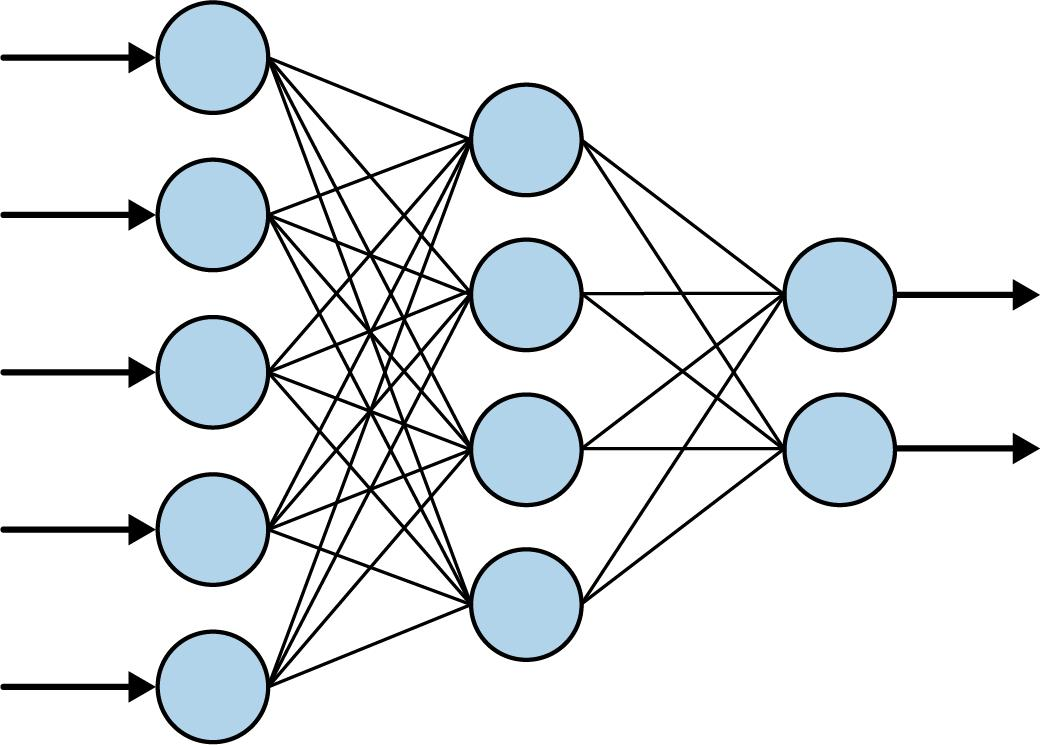
\includegraphics[width=0.7\textwidth]{capitulo3/neurona.jpg}
	\caption{Estructura de la red neuronal}
	\label{cap3:005}
\end{figure}

Cuando vea una red neuronal como esta, considere cada uno de los "círculos" como una neurona y cada una de las columnas de círculos como una capa. Entonces, en la Figura \ref{cap3:005}, hay tres capas: la primera tiene cinco neuronas, la segunda tiene cuatro y la tercera tiene dos.

Si miramos hacia atrás en nuestro código y observamos solo la primera línea, veremos que estamos definiendo la red neuronal más simple posible. Solo hay una capa, y contiene solo una neurona:

\begin{lstlisting}[language=python]
modelo = Sequential([Dense(units=1, input_shape=[1])])
\end{lstlisting}

Cuando usa TensorFlow, define sus capas usando Sequential. Dentro de Sequential, luego especifica cómo se ve cada capa. Solo tenemos una línea dentro de nuestro secuencial, por lo que solo tenemos una capa. Luego define cómo se ve la capa usando la API keras.layers. Hay muchos tipos de capas diferentes, pero aquí estamos usando una capa Densa. "Densa" significa un conjunto de neuronas completamente (o densamente) conectadas, que es lo que puede ver en la Figura \ref{cap3:005}, donde cada neurona está conectada a cada neurona en la siguiente capa. Es la forma más común de tipo de capa. Nuestra capa densa tiene unidades = 1 especificadas, por lo que solo tenemos una capa densa con una neurona en toda nuestra red neuronal. Finalmente, cuando especifica la primera capa en una red neuronal (en este caso, es nuestra única capa), debe decirle cuál es la forma de los datos de entrada. En este caso, nuestros datos de entrada son nuestra X, que es solo un valor, por lo que especificamos que esa es su forma. La siguiente línea es donde realmente comienza la diversión. Veámoslo de nuevo:

\begin{lstlisting}[language=python]
modelo.compile(optimizer='sgd', loss='mean_squared_error')
\end{lstlisting}

Si ha hecho algo con el aprendizaje automático antes, probablemente haya visto que involucra muchas matemáticas. Si no ha hecho cálculo en años, podría haberle parecido una barrera de entrada. Aquí está la parte donde entran las matemáticas: es el núcleo del aprendizaje automático. En un escenario como este, la computadora no tiene idea de cuál es la relación entre X e Y. Así que hará una conjetura. Digamos, por ejemplo, que adivina que Y = 10X + 10. Luego necesita medir cuán buena o mala es esa suposición. Ese es el trabajo de la función de pérdida. Ya conoce las respuestas cuando X es –1, 0, 1, 2, 3 y 4, por lo que la función de pérdida puede compararlas con las respuestas de la relación adivinada. Si adivinó Y = 10X + 10, entonces cuando X es -1, Y será 0. La respuesta correcta era -3, por lo que está un poco equivocado. Pero cuando X es 4, la respuesta adivinada es 50, mientras que la correcta es 7. Eso está muy lejos. Armado con este conocimiento, la computadora puede hacer otra conjetura. Ese es el trabajo del optimizador. Aquí es donde se usa el cálculo pesado, pero con TensorFlow, eso se puede ocultar. Simplemente elija el optimizador apropiado para usar en diferentes escenarios. En este caso, elegimos uno llamado sgd, que significa descenso de gradiente estocástico, una función matemática compleja que, cuando se le dan los valores, la suposición anterior y los resultados de calcular los errores (o pérdidas) en esa suposición, puede generar otra una. Con el tiempo, su trabajo es minimizar la pérdida y, al hacerlo, acercar más y más la fórmula adivinada a la respuesta correcta. A continuación, simplemente formateamos nuestros números en el formato de datos que esperan las capas. En Python, hay una biblioteca llamada Numpy que TensorFlow puede usar, y aquí ponemos nuestros números en una matriz Numpy para que sea más fácil procesarlos:

\begin{lstlisting}[language=python]
	xs = np.array([-1.0, 0.0, 1.0, 2.0, 3.0, 4.0], dtype=float)
	ys = np.array([-3.0, -1.0, 1.0, 3.0, 5.0, 7.0], dtype=float)
\end{lstlisting}

El proceso de aprendizaje comenzará con el comando model.fit, así:

\begin{lstlisting}[language=python]
modelo.fit(xs, ys, epochs=1000)
\end{lstlisting}

Puede leer esto como ``ajustar las X a las Y e intentarlo 1000 veces''. Entonces, en el primer intento, la computadora adivinará la relación (es decir, algo como Y = 10X + 10) y medirá qué tan buena o mala fue esa suposición. Luego enviará esos resultados al optimizador, que generará otra suposición. Luego, este proceso se repetirá, con la lógica de que la pérdida (o el error) disminuirá con el tiempo y, como resultado, la ``suposición'' será cada vez mejor.

Ahora podemos ver que la pérdida es de 2,61 × 10-5. La pérdida se ha vuelto tan pequeña que el modelo prácticamente ha descubierto que la relación entre los números es \textbf{Y = 2X – 1}. La máquina ha aprendido el patrón entre ellos. Nuestra última línea de código usó el modelo entrenado para obtener una predicción como esta:

\begin{lstlisting}[language=python]
print(modelo.predict([10.0]))
\end{lstlisting}

El término predicción se usa típicamente cuando se trata de modelos ML. ¡Sin embargo, no pienses en ello como mirar hacia el futuro! Este término se usa porque estamos lidiando con una cierta cantidad de incertidumbre. Piense en el escenario de detección de actividad del que hablamos anteriormente. Cuando la persona se movía a cierta velocidad, probablemente estaba caminando. De manera similar, cuando un modelo aprende acerca de los patrones entre dos cosas, nos dirá cuál es probablemente la respuesta. En otras palabras, es predecir la respuesta. (Más adelante también aprenderá sobre la inferencia, donde el modelo elige una respuesta entre muchas e infiere que ha elegido la correcta).

¿Cuál crees que será la respuesta cuando le pidamos al modelo que prediga Y cuando X es 10? Podrías pensar instantáneamente en 19, pero eso no es correcto. Elegirá un valor muy cercano a 19. Esto se debe a varias razones. En primer lugar, nuestra pérdida no fue 0. Todavía era una cantidad muy pequeña, por lo que deberíamos esperar que cualquier respuesta prevista se desviara por una cantidad muy pequeña. En segundo lugar, la red neuronal se entrena solo con una pequeña cantidad de datos; en este caso, solo seis pares de valores (X, Y).

El modelo solo tiene una sola neurona, y esa neurona aprende un peso y un sesgo, de modo que Y = WX + B. Esto se ve exactamente como la relación \textbf{Y = 2X – 1} que queremos, donde nos gustaría que aprendiera que W = 2 y B = –1. Dado que el modelo se entrenó en solo seis elementos de datos, nunca se podría esperar que la respuesta fuera exactamente estos valores, sino algo muy cercano a ellos. Ejecute el código usted mismo para ver lo que obtiene. Obtuve 18.977888 cuando lo ejecuté, pero su respuesta puede diferir ligeramente porque cuando la red neuronal se inicializa por primera vez, hay un elemento aleatorio: su suposición inicial será ligeramente diferente de la mía y de la de una tercera persona.

\section{Ver lo que aprendió la red}

Obviamente, este es un escenario muy simple, donde estamos emparejando \textbf{Xs} con \textbf{Ys} en una relación lineal. Como se mencionó en la sección anterior, las neuronas tienen parámetros de peso y sesgo que aprenden, lo que hace que una sola neurona esté bien para aprender una relación como esta: a saber, cuando \textbf{Y = 2X – 1}, el peso es 2 y el sesgo es –1. Con \textbf{TensorFlow}, podemos echar un vistazo a los pesos y sesgos que se aprenden, con un simple cambio en nuestro código como este:

\begin{lstlisting}[language=python]
import tensorflow as tf
import numpy as np
from tensorflow.keras import Sequential
from tensorflow.keras.layers import Dense

l0 = Dense(units=1, input_shape=[1])
modelo = Sequential([l0])
modelo.compile(optimizer='sgd', loss='mean_squared_error')

xs = np.array([-1.0, 0.0, 1.0, 2.0, 3.0, 4.0], dtype=float)
ys = np.array([-3.0, -1.0, 1.0, 3.0, 5.0, 7.0], dtype=float)

modelo.fit(xs, ys, epochs=1000)

print(modelo.predict([10.0]))
print("Aqui esta lo que aprendi: {}".format(l0.get_weights()))
\end{lstlisting}

La diferencia es que creé una variable llamada l0 para contener la capa densa. Luego, después de que la red termine de aprender, puedo imprimir los valores (o pesos) que aprendió la capa.
